\chapter{Monte Carlo Simulation}
\label{appendix:montecarlo}

The error of the optimized results can be estimated 
from Monte Carlo simulation for both statistical deviation as well as 
taking the systematical error from the apparatus into account
as the total error.

Since the complexity in the heuristic optimizations much higher 
than the plain gradient descent method. In this simulation 
for estimating the deviation, the optimization process is conducted
from applying the gradient descent method with a given global 
optimized results. The distribution outcome of each parameter will be
fitted for finding the deviation via normal distribution function. 
The mean value of the function will be fixed by the best global 
optimization.


\begin{figure}[h!]
    \centering
        \subfloat[
            Statistical deviation
        ]{
            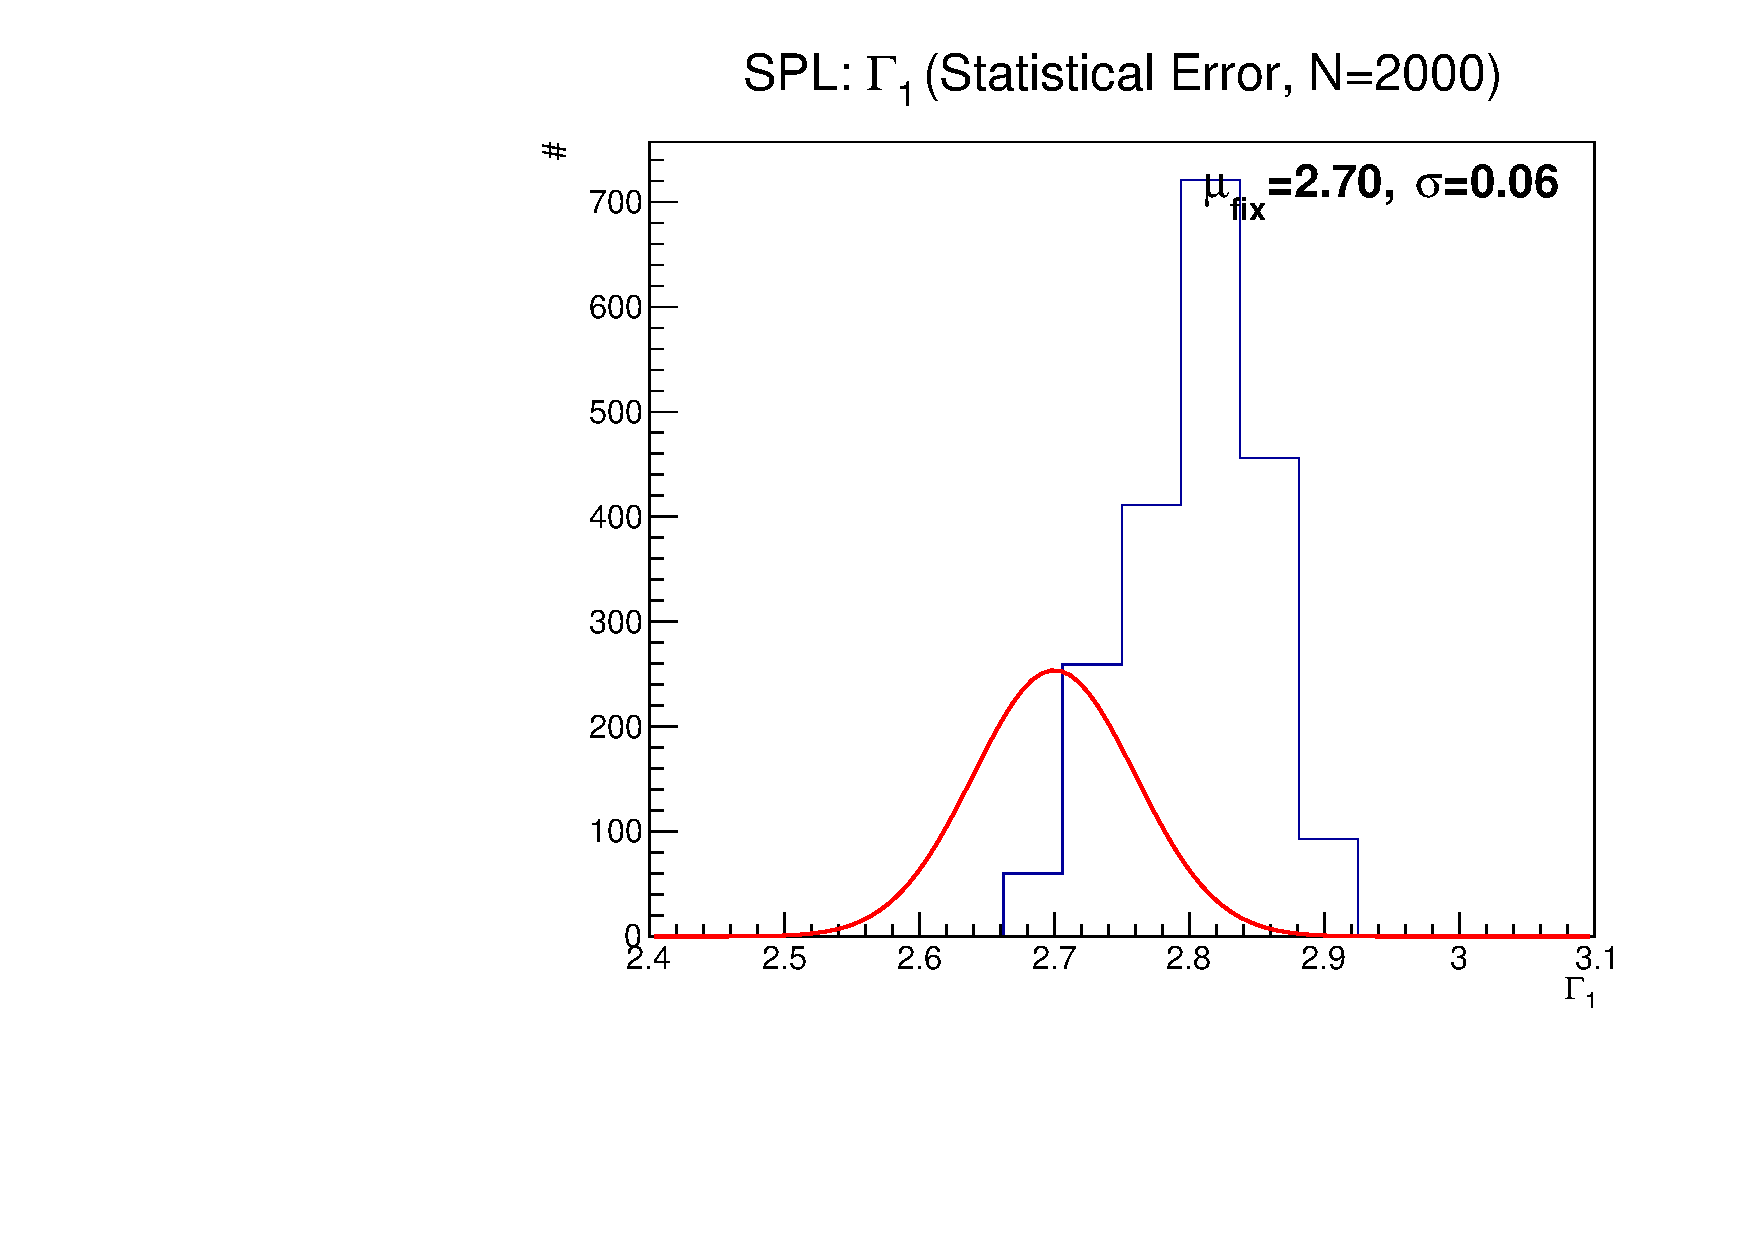
\includegraphics[width=0.48\textwidth]{appendix/montecarlo/figures/SPLwHe_gamma1_sys.pdf}
            }
        \hfill
         \subfloat[
            Total deviation
         ]{
            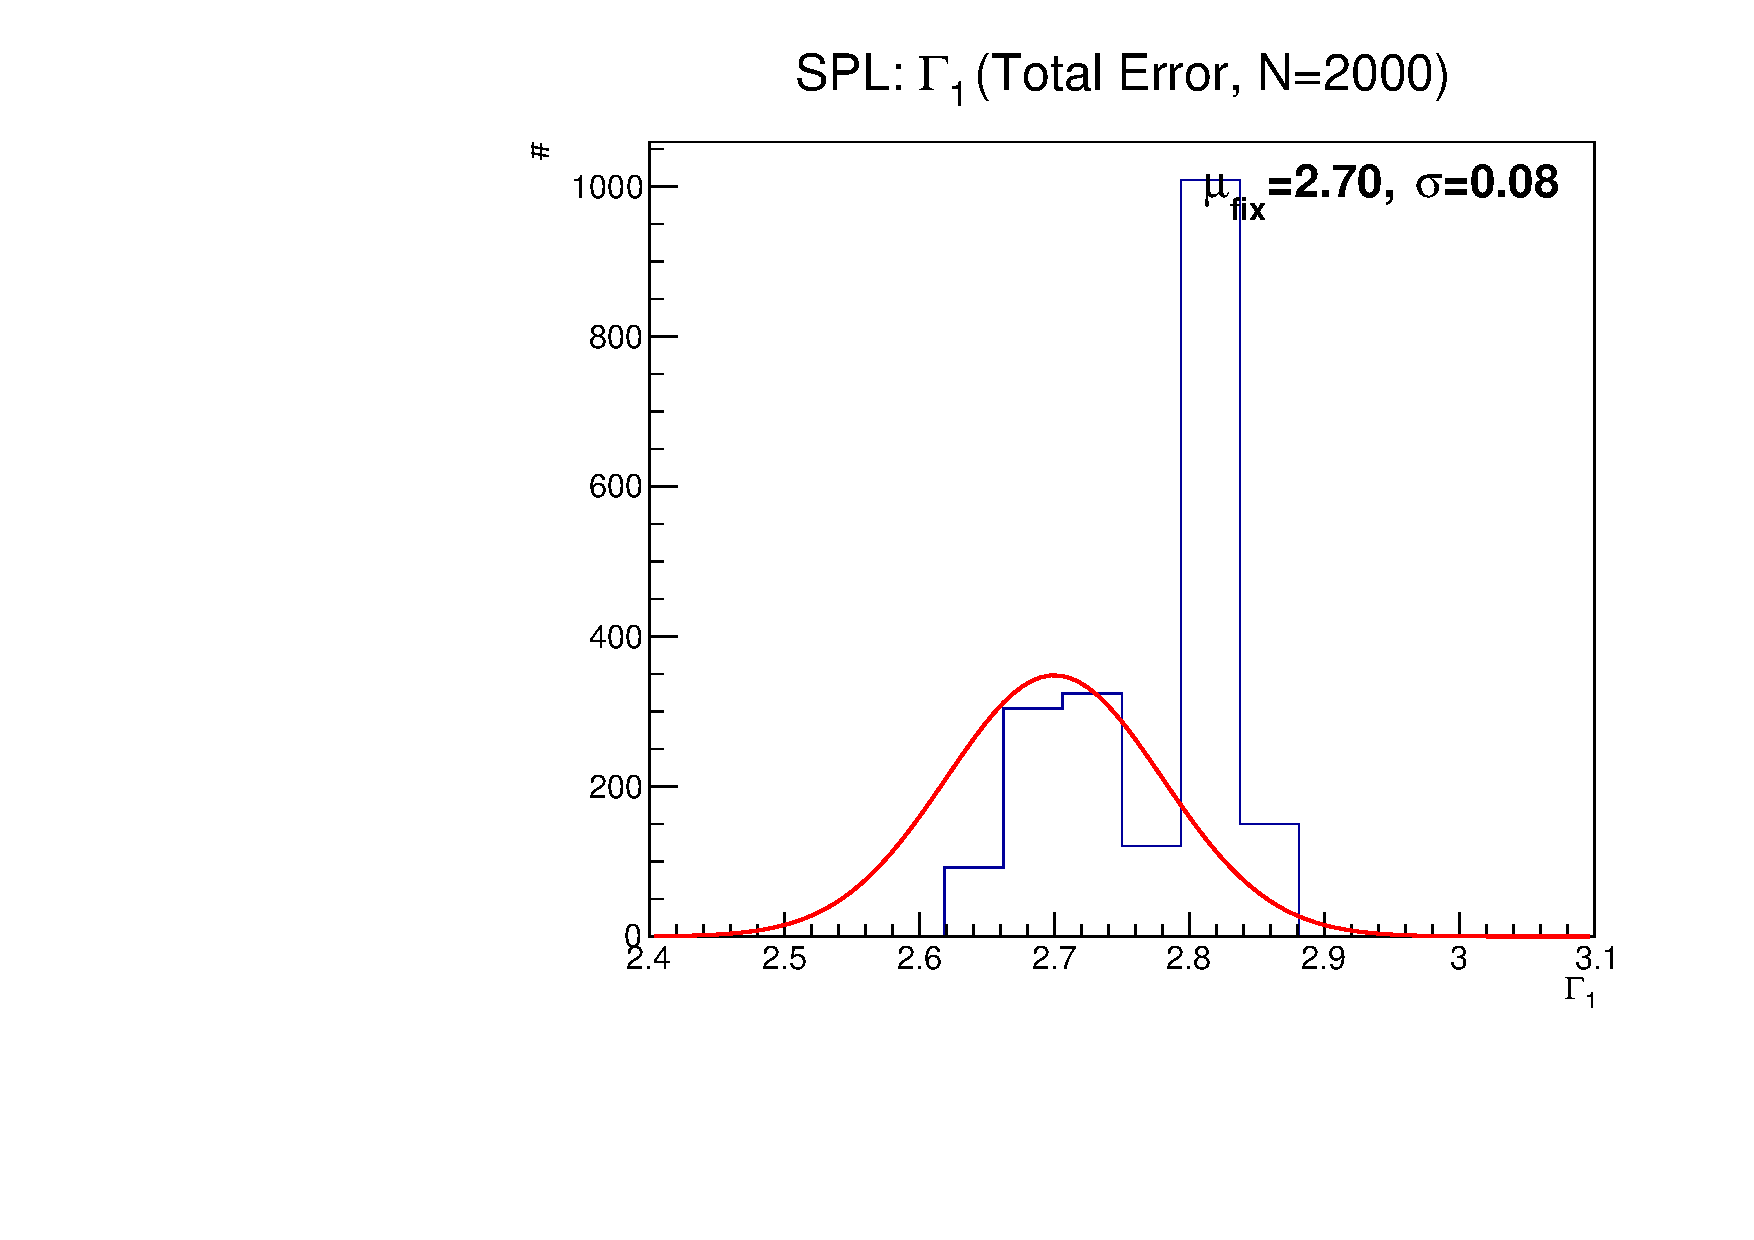
\includegraphics[width=0.48\textwidth]{appendix/montecarlo/figures/SPLwHe_gamma1_tot.pdf}
        }
        \caption{
            The distribution of the fitted results by SPL model
            from the distortion.
        }
       \label{fig:monte_spl}
\end{figure}

Simulation process for statistical deviation is done by 
rescaling the spectrum from the information of the arrival photon.
The discrete probability of the events from a fixed amount
of time could be modeled by using poisson distribution function.
Hence, the photon spectrum in each energy bin will be rescaled
by resampling photon numbers from a given amount of photon 
from observations as the number of occurrences.

The results from the statistical simulation for SPL is shown in 
Figure \ref{fig:monte_spl}a as well as Figure \ref{fig:monte_bpl_stat}
demonstrates the deviation of BPL model.

\begin{figure}[h!]
    \centering
        \subfloat[First spectral index]{
            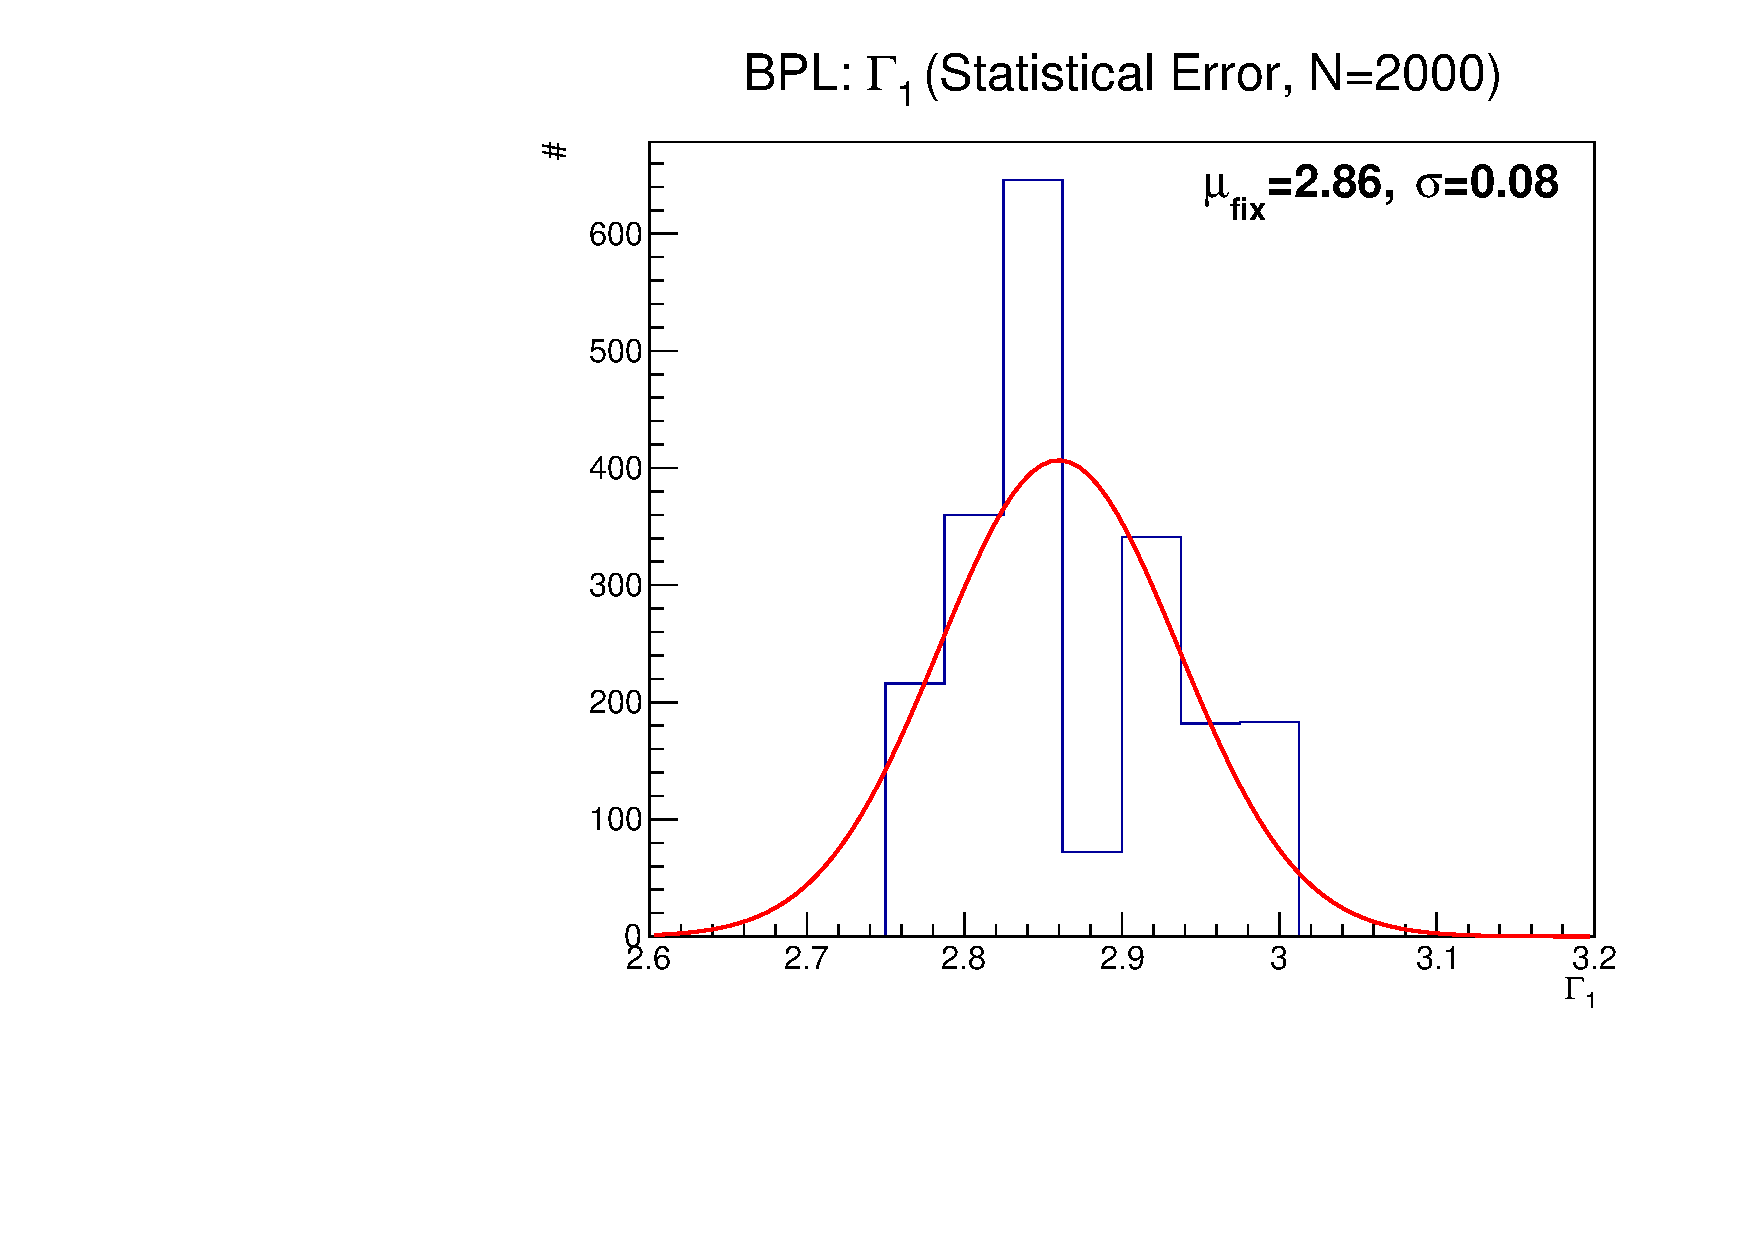
\includegraphics[width=0.33\textwidth]{appendix/montecarlo/figures/BPLwHe_gamma1_sys.pdf}
        }
        \subfloat[Second spectral index]{
            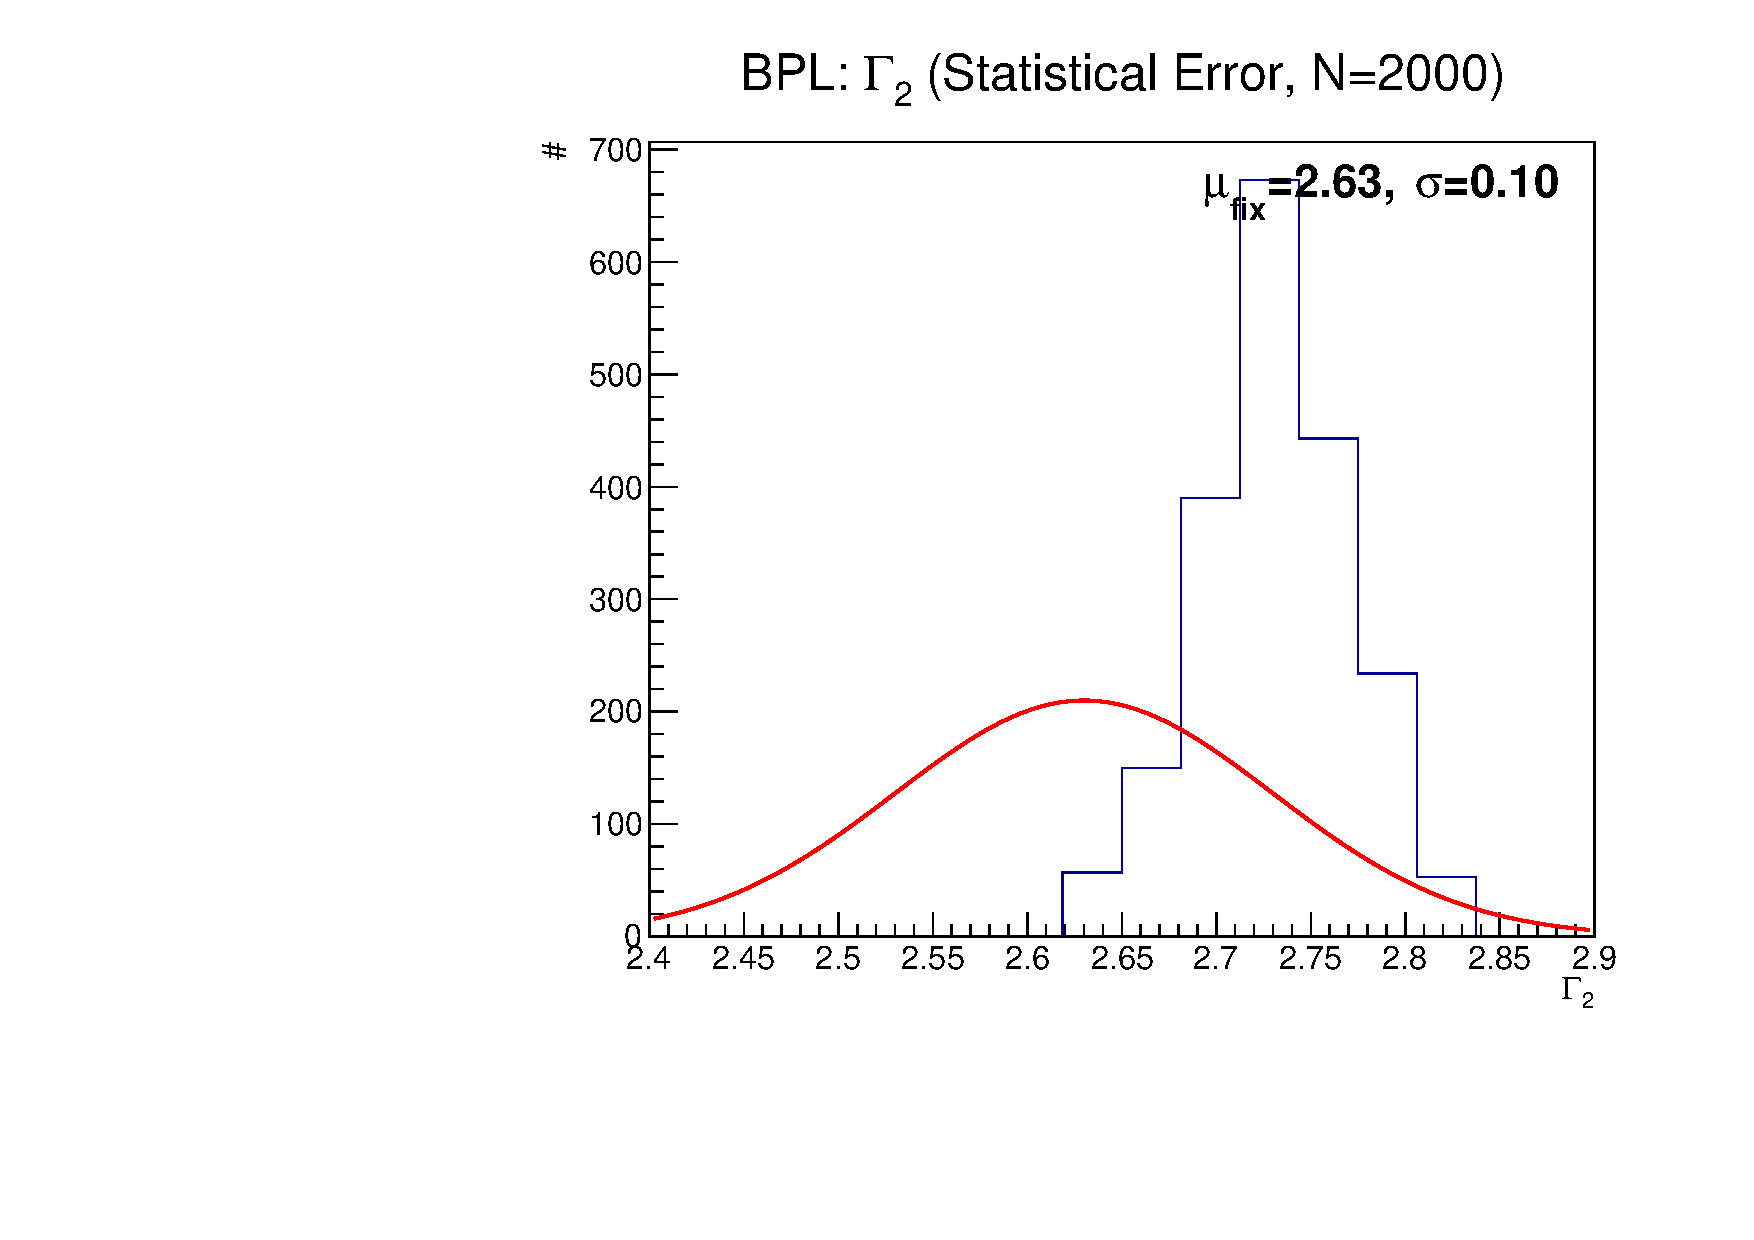
\includegraphics[width=0.33\textwidth]{appendix/montecarlo/figures/BPLwHe_gamma2_sys.pdf}
        }
        \subfloat[Breaking energy]{
            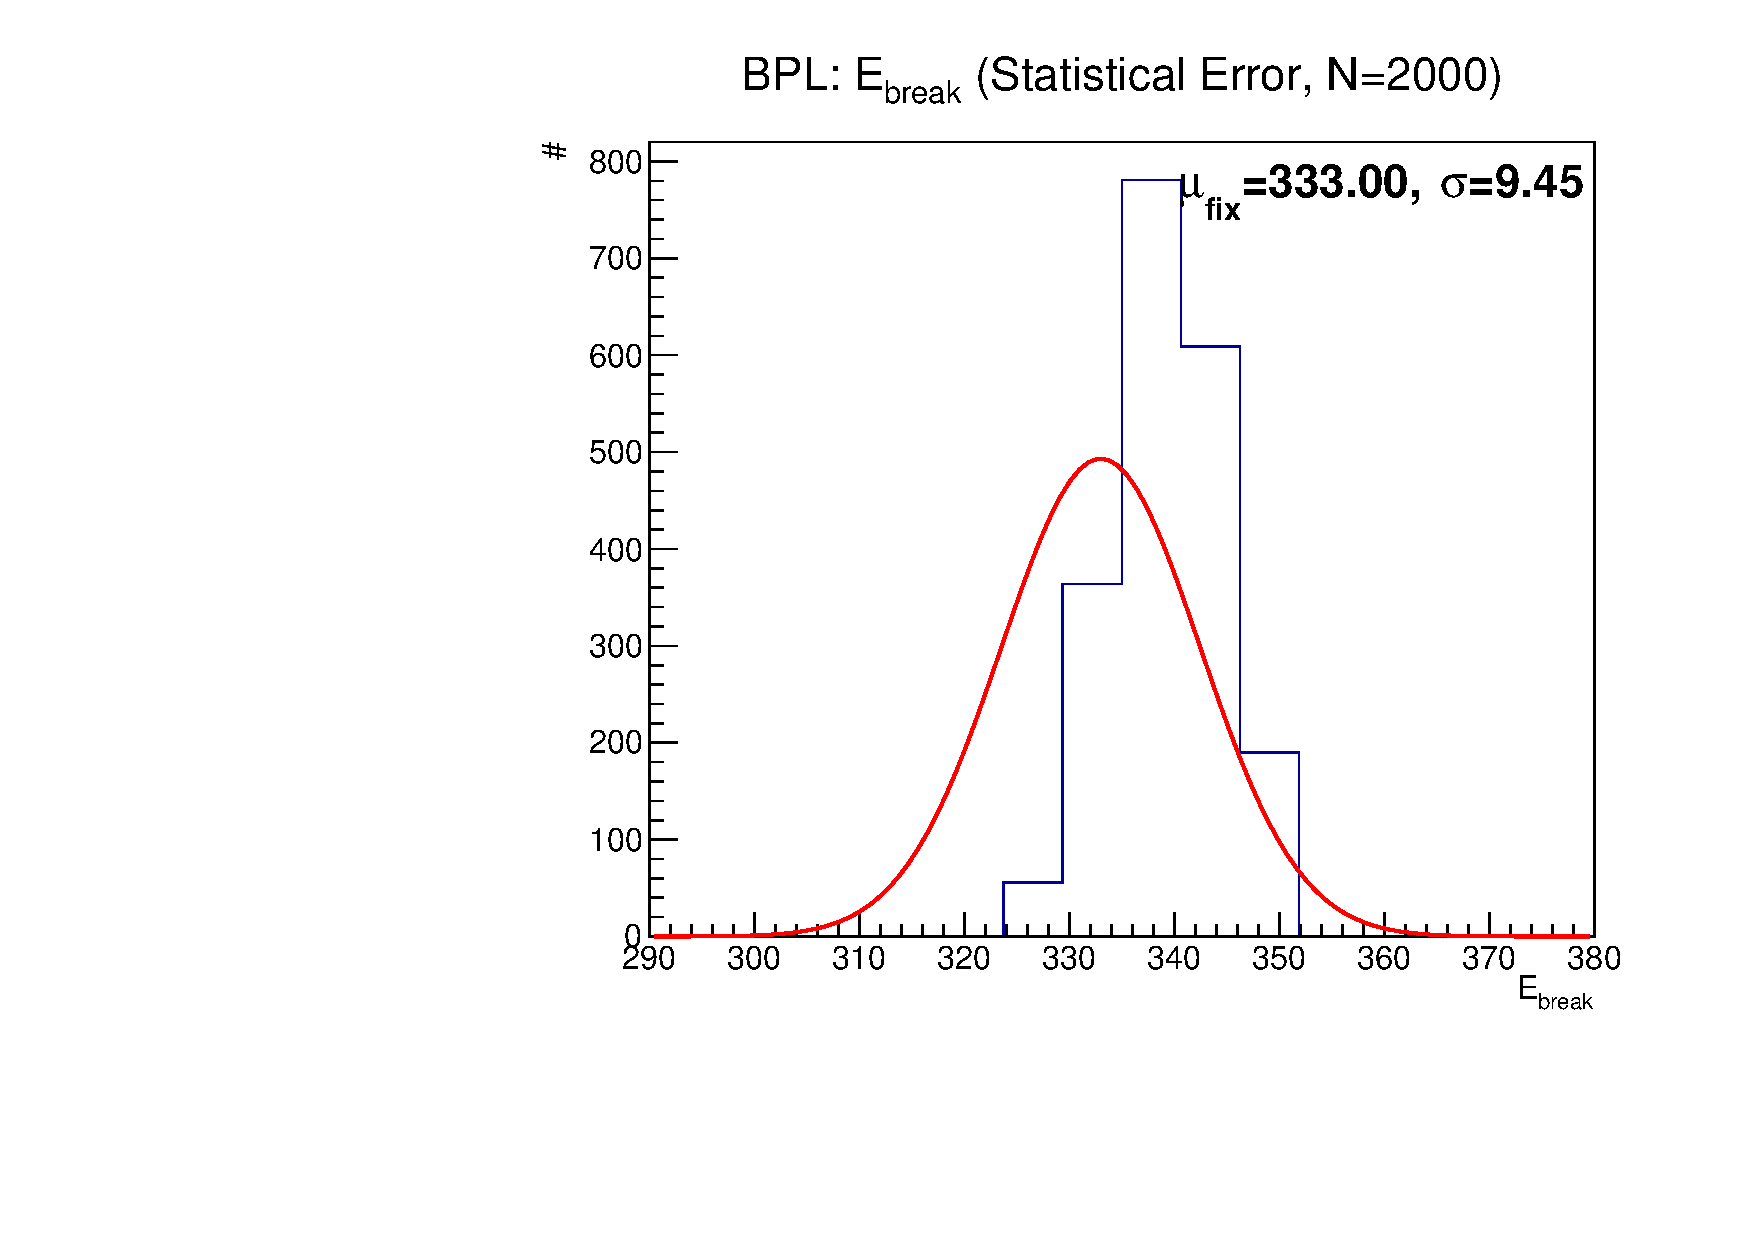
\includegraphics[width=0.33\textwidth]{appendix/montecarlo/figures/BPLwHe_e_break_sys.pdf}
        }        
        \caption{Statistical simulation of the BPL model}
       \label{fig:monte_bpl_stat}
\end{figure}

On the other hand, total deviation is taken the systematical distortion
into account. It is modeled as an uncertain from the detector\footnote{\url{https://fermi.gsfc.nasa.gov/ssc/data/analysis/scitools/Aeff_Systematics.html}}.
First step for generating spectrum is exactly the same as the 
statistical error. The following step is to purturb the spectrum
by the distorted curved. The curved is computed by sample three 
different points in 3 energy decades (10 GeV, 100 GeV and 1 TeV).


The results of the total error of SPL model is illustrated in
Figure \ref{fig:monte_spl}b and the deviation of the BPL parameters
is shown in Figure \ref{fig:monte_bpl_tot}.

\begin{figure}[h!]
    \centering
        \subfloat[First spectral index]{
            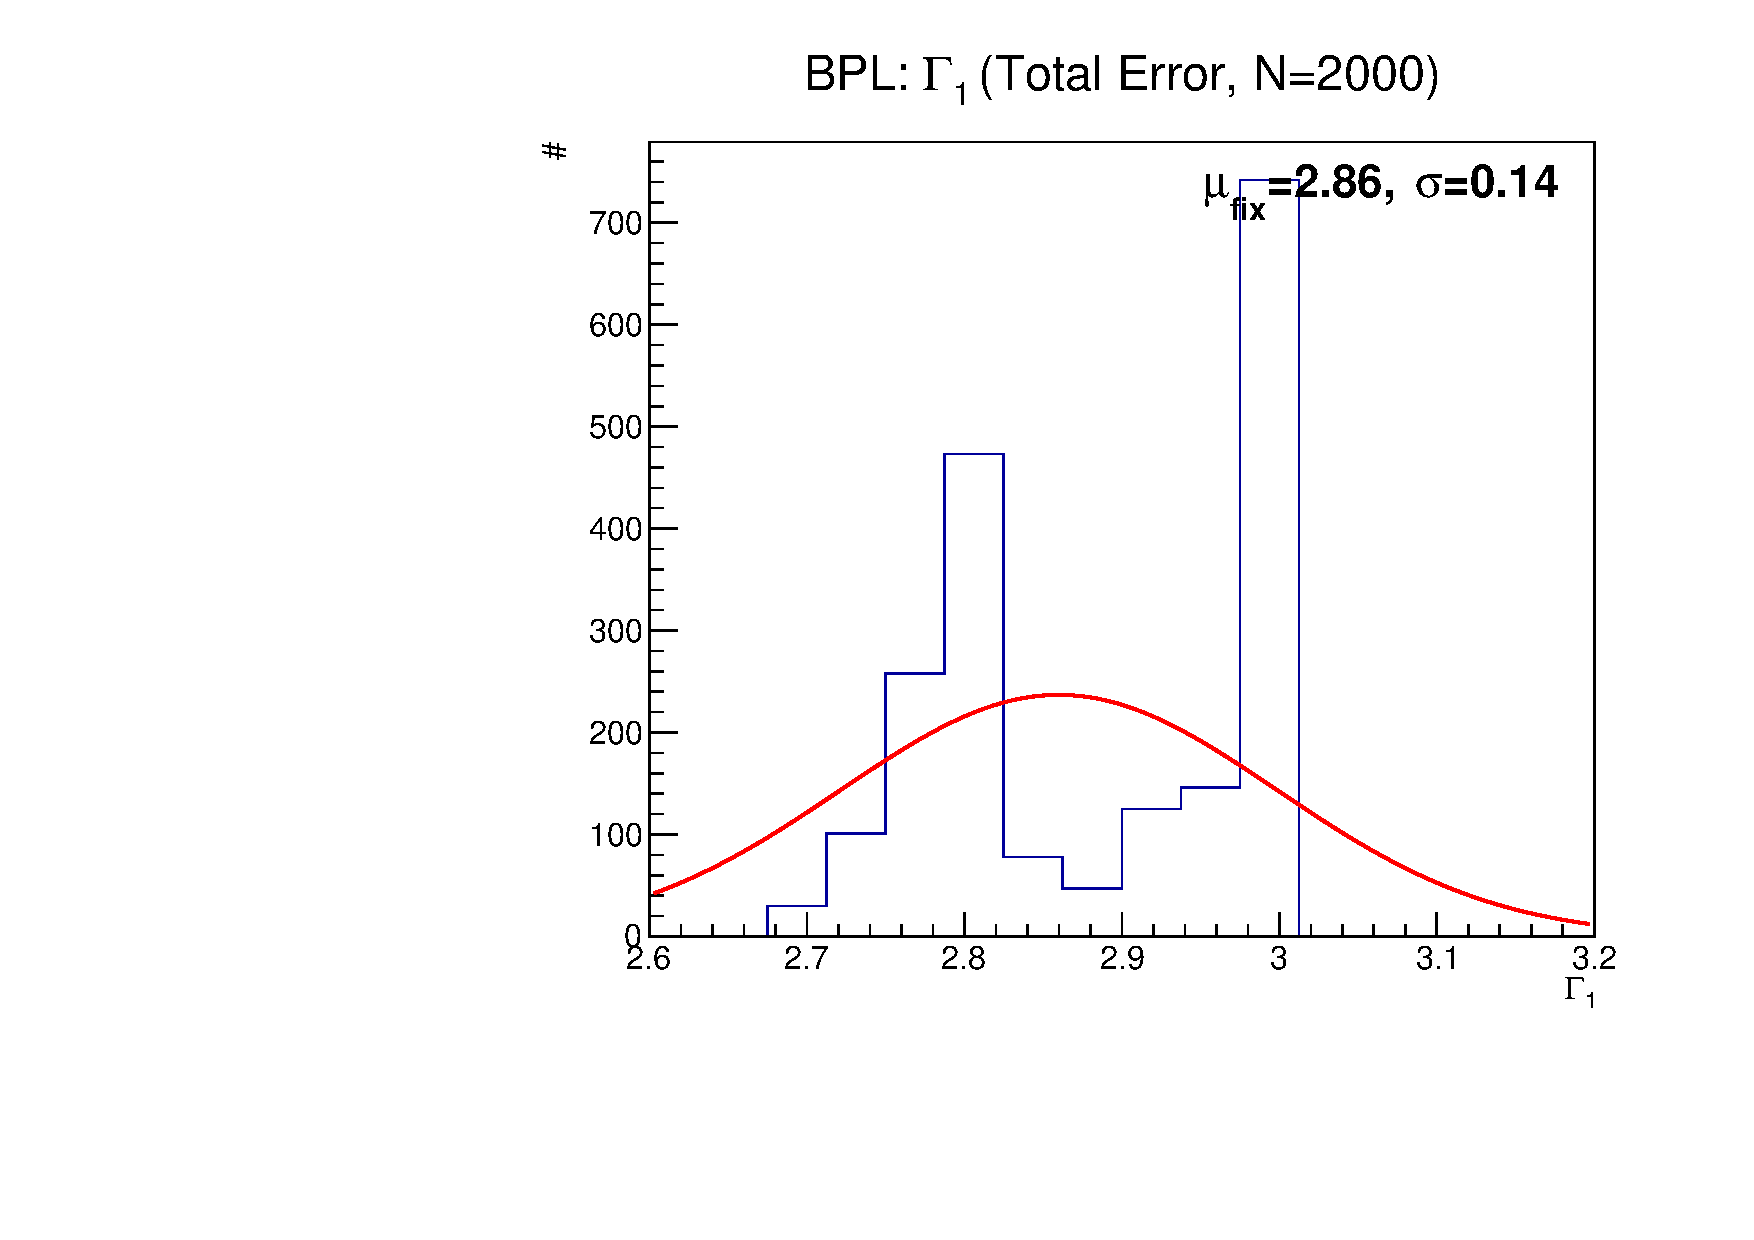
\includegraphics[width=0.33\textwidth]{appendix/montecarlo/figures/BPLwHe_gamma1_tot.pdf}
        }
        \subfloat[Second spectral index]{
            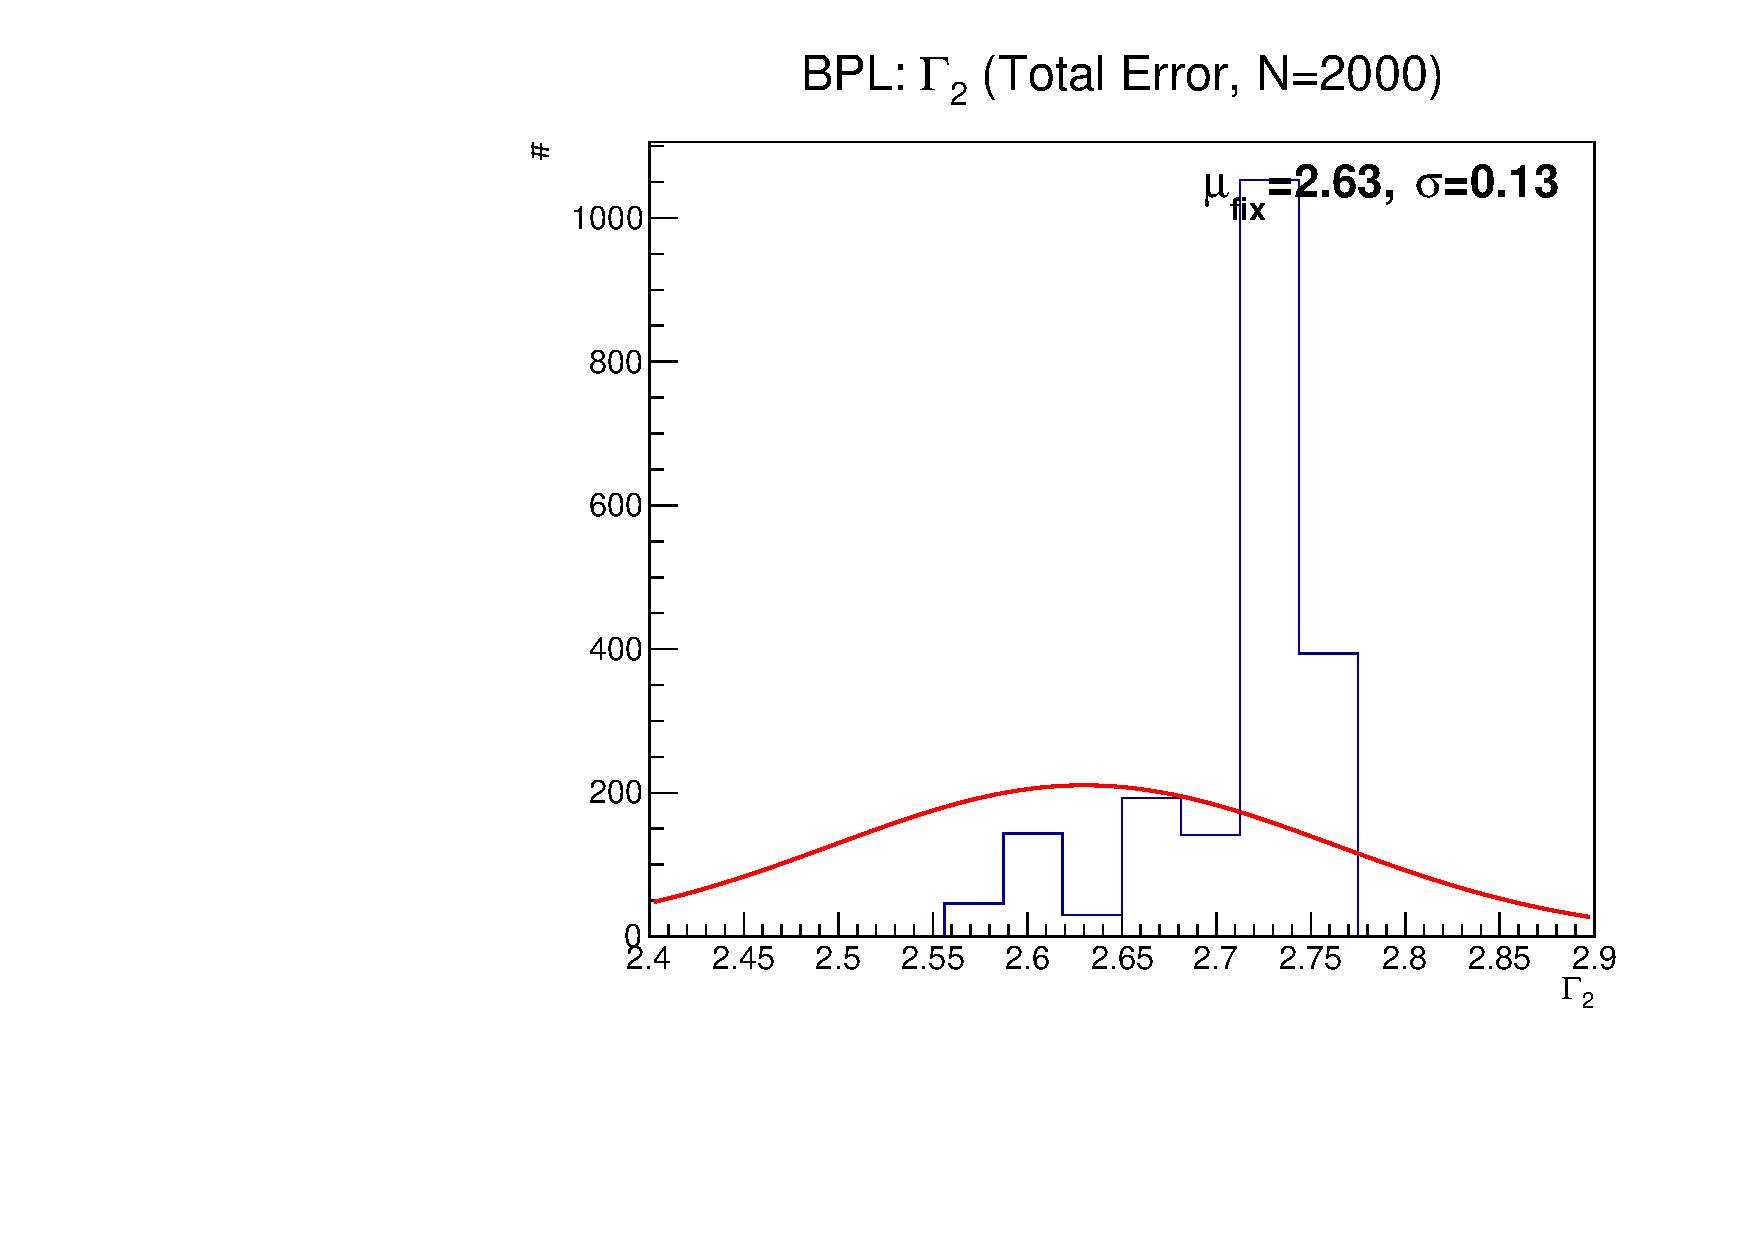
\includegraphics[width=0.33\textwidth]{appendix/montecarlo/figures/BPLwHe_gamma2_tot.pdf}
        }
        \subfloat[Breaking energy]{
            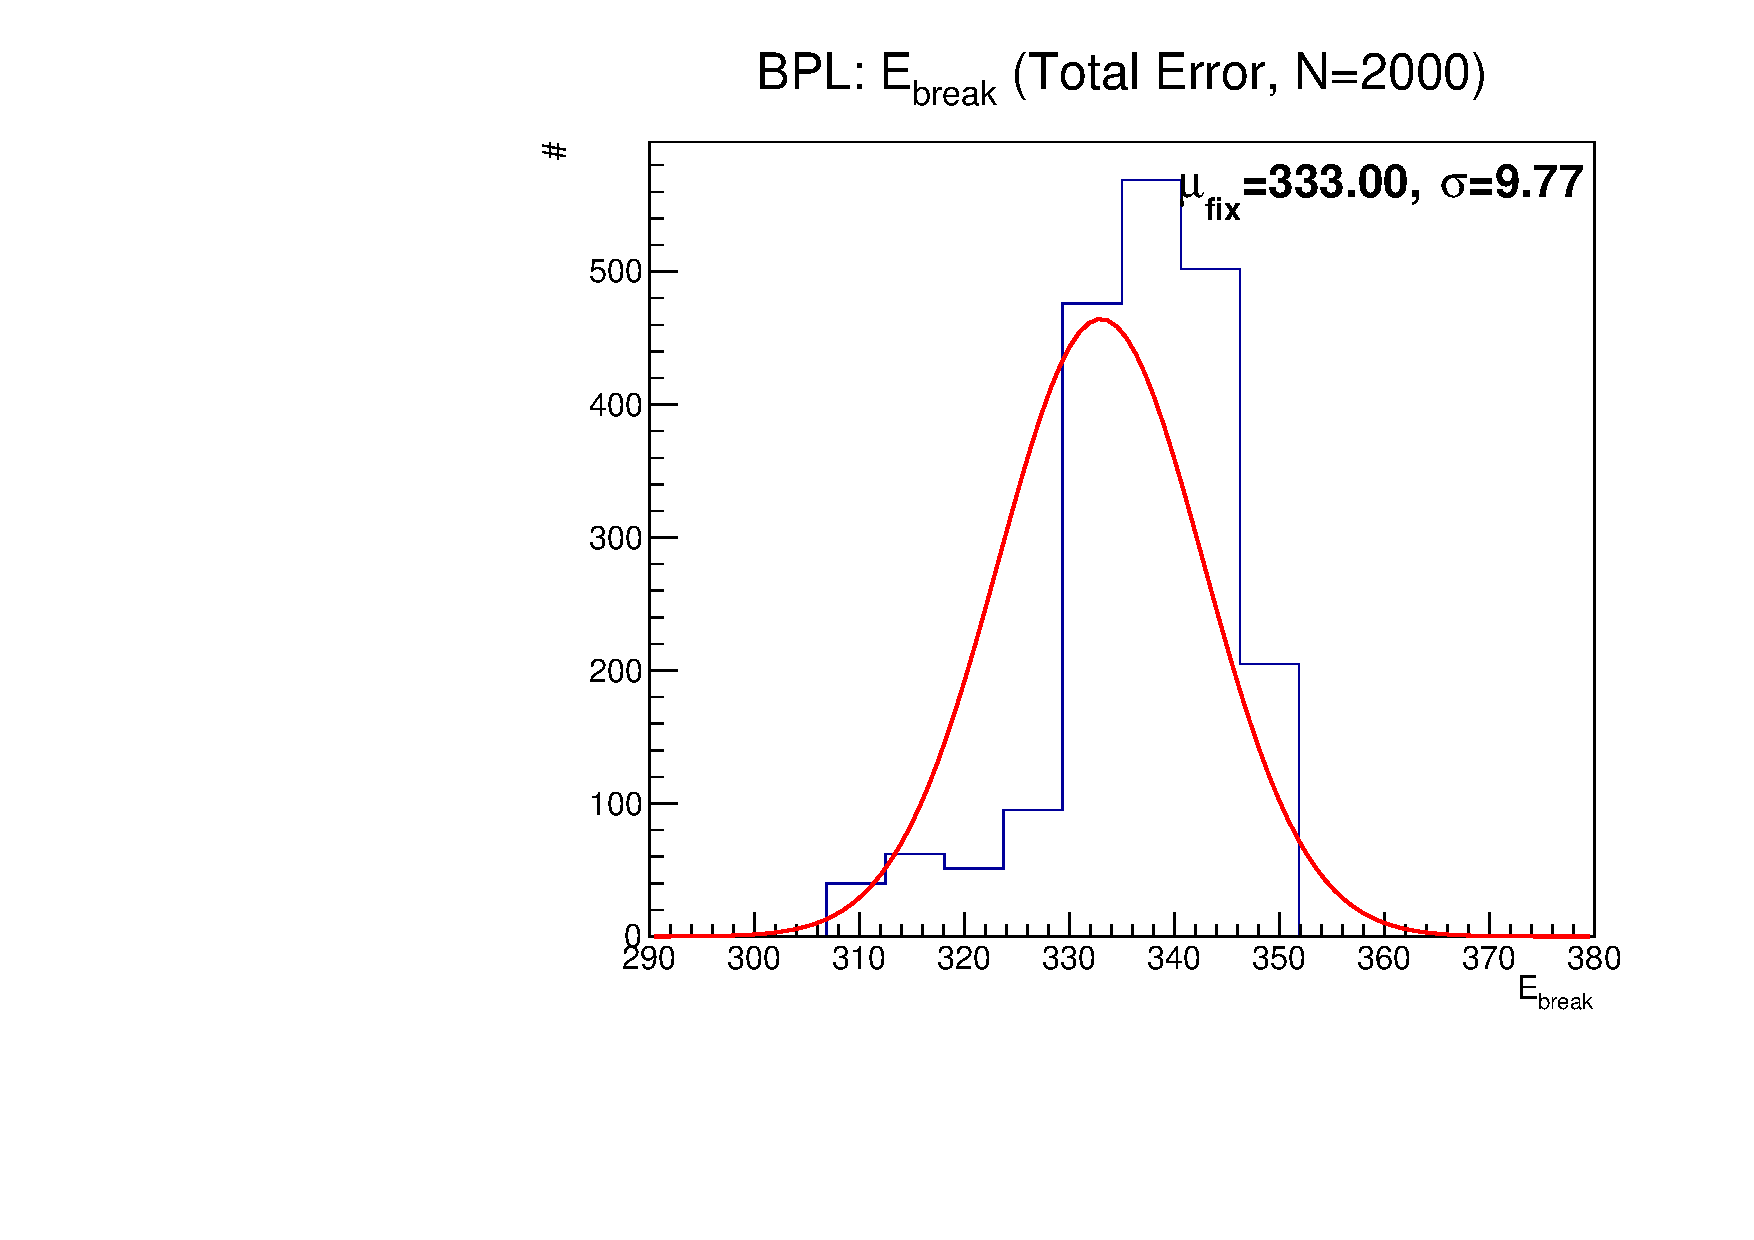
\includegraphics[width=0.33\textwidth]{appendix/montecarlo/figures/BPLwHe_e_break_tot.pdf}
        }        
        \caption{Statistical and systematical (Total) simulation of the BPL model}
       \label{fig:monte_bpl_tot}
\end{figure}